\documentclass[main.tex]{subfiles}
\begin{document}\newpage
\setdoublesep{0.35700 em}  % 'Bond Spacing'
\setatomsep{1.78500 em}    % 'Fixed Length'
\setbondoffset{0.18265 em} % 'Margin Width'
\newcommand{\bondwidth}{0.06642 em} % 'Line Width'
\setbondstyle{line width = \bondwidth}
\newgeometry{left=0.8in,right=0.8in, top=2.5cm,bottom=2cm}
\fancyhfoffset[E,O]{0pt}
\setlength{\columnsep}{30pt}
\begin{conclusion}
\end{conclusion}
%\setstretch{0.3}
\begin{multicols*}{2}\setcounter{numA}{1}

{\raggedright\textsc{\textbf{Spontaneity and entropy}}\par}


\begin{question}[ID=\the\value{numA}]\SetQuestionProperties{section-title=\nameref{sec:units}}
Which of the following processes are spontaneous:
\begin{inparaenum}[(a)]
\item An apple falls down a tree % (spontaneous)
\item Water flowing down a river % (spontaneous)
\item Water flowing up a river % (nonspontaneous)
\item A ball rolling downhill % (spontaneous)
 \end{inparaenum}
\end{question}
\begin{solution}
\begin{inparaenum}[(a)]
\item An apple falls down a tree   (spontaneous)
\item Water flowing down a river   (spontaneous)
\item Water flowing up a river   (nonspontaneous)
\item A ball rolling downhill   (spontaneous)
\end{inparaenum}
\hspace{0.1cm}\end{solution}\stepcounter{numA}%%%%%%%%%%%%

\begin{question}[ID=\the\value{numA}]\SetQuestionProperties{section-title=\nameref{sec:units}}
Which of the following processes are spontaneous:
\begin{inparaenum}[(a)]
\item A ball rolling uphill % (nonspontaneous)
\item Sugar dissolving on coffe % (spontaneous)
\item Cacao powder dissolving in cold water % (nonspontaneous)
\item An iron pipe rusting % (spontaneous)
 \end{inparaenum}
\end{question}
\begin{solution}
\begin{inparaenum}[(a)]
\item A ball rolling uphill   (nonspontaneous)
\item Sugar dissolving on coffe   (spontaneous)
\item Cacao powder dissolving in cold water   (nonspontaneous)
\item An iron pipe rusting   (spontaneous)
\end{inparaenum}
\hspace{0.1cm}\end{solution}\stepcounter{numA}%%%%%%%%%%%%


\begin{question}[ID=\the\value{numA}]\SetQuestionProperties{section-title=\nameref{sec:units}}
Which of the following processes are spontaneous:
\begin{inparaenum}[(a)]
\item Boiling of water at 100$^{\circ}$C and 1atm % (spontaneous)
\item Boiling of water at 50$^{\circ}$C and 1atm % (nonspontaneous)
\item Boiling of water at 100$^{\circ}$C and 2atm % (nonspontaneous)
\item Melting of ice at 0$^{\circ}$C % (spontaneous)
\item Melting of ice at 10$^{\circ}$C % (nonspontaneous)
 \end{inparaenum}
\end{question}
\begin{solution}
\begin{inparaenum}[(a)]
\item Boiling of water at 100$^{\circ}$C and 1atm  (spontaneous)
\item Boiling of water at 50$^{\circ}$C and 1atm   (nonspontaneous)
\item Boiling of water at 100$^{\circ}$C and 2atm   (nonspontaneous)
\item Melting of ice at 0$^{\circ}$C   (spontaneous)
\item Melting of ice at 10$^{\circ}$C   (nonspontaneous)
\end{inparaenum}
\hspace{0.1cm}\end{solution}\stepcounter{numA}%%%%%%%%%%%%




\begin{question}[ID=\the\value{numA}]\SetQuestionProperties{section-title=\nameref{sec:units}}
Think about the possible arrangements of two identical molecules in a two-bulbed flask:
\begin{center}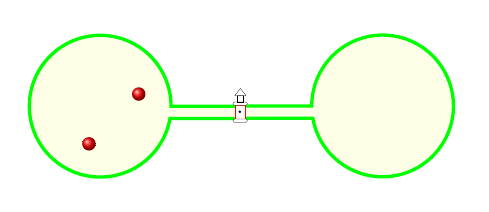
\begin{tikzpicture}[thick,scale=0.9, every node/.style={transform shape}]
\draw [green, very thick,  fill=yellow!10] (0,0) -- ++ (-1,0) arc (0:350:1.0) -- ++ (1,0)   |- cycle ;
\draw [green, very thick,  fill=yellow!10, yshift=.83cm]  (0,-1)-- ++(1,0) arc (190:540:1.0)  -- ++(-1,0)|- cycle ;
\begin{scope}[transform canvas={scale=.1},overlay,shift={(-1,-1.8)}]
\draw [red, fill=white] (0,0) -- ++ (1.5,0)-- ++ (0,1.9)-- ++ (-1.5,0)   |- cycle ;
\draw[rounded corners=5pt, fill=white] (-0.25,1.9) rectangle ++(2,0.5);
\draw[rounded corners=5pt, fill=white] (-0.25,-.5) rectangle ++(2,0.5);
\draw (.7,1) node[circle, draw,fill=black]{};
\draw[xshift=9, yshift=1.4cm]  (0,1) rectangle ++(.8,1);
\draw [black, fill=white,yshift=3.3cm, xshift=-.5] (0,0) -- ++ (.8,1)-- ++ (.8,-1)    |- cycle ;
\shade [ball color=red, shift={(-40em,10em)}] (0:0.5) circle (0.95cm);
\shade [ball color=red, shift={(-60em,-10em)}] (0:0.5) circle (0.95cm);
\end{scope}
\end{tikzpicture}\end{center}
\begin{inparaenum}[(a)]
\item How many arrangements are possible?	%(3)
\item Which is the most likely arrangement?	%(spread circles)
\item Which is the probability of the most likely arrangement?	%(0.33)
\end{inparaenum}
\end{question}
\begin{solution}
\begin{inparaenum}[(a)]
\item  3 
\item  spread circles 
\item  0.33 
\end{inparaenum}
\hspace{0.1cm}\end{solution}\stepcounter{numA}%%%%%%%%%%%%



\begin{question}[ID=\the\value{numA}]\SetQuestionProperties{section-title=\nameref{sec:units}}
Think about the possible arrangements of two different molecules in a two-bulbed flask:
\begin{center}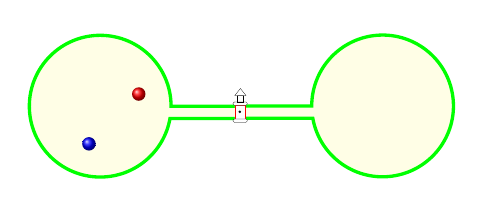
\begin{tikzpicture}[thick,scale=0.9, every node/.style={transform shape}]
\draw [green, very thick,  fill=yellow!10] (0,0) -- ++ (-1,0) arc (0:350:1.0) -- ++ (1,0)   |- cycle ;
\draw [green, very thick,  fill=yellow!10, yshift=.83cm]  (0,-1)-- ++(1,0) arc (190:540:1.0)  -- ++(-1,0)|- cycle ;
\begin{scope}[transform canvas={scale=.1},overlay,shift={(-1,-1.8)}]
\draw [red, fill=white] (0,0) -- ++ (1.5,0)-- ++ (0,1.9)-- ++ (-1.5,0)   |- cycle ;
\draw[rounded corners=5pt, fill=white] (-0.25,1.9) rectangle ++(2,0.5);
\draw[rounded corners=5pt, fill=white] (-0.25,-.5) rectangle ++(2,0.5);
\draw (.7,1) node[circle, draw,fill=black]{};
\draw[xshift=9, yshift=1.4cm]  (0,1) rectangle ++(.8,1);
\draw [black, fill=white,yshift=3.3cm, xshift=-.5] (0,0) -- ++ (.8,1)-- ++ (.8,-1)    |- cycle ;
\shade [ball color=red, shift={(-40em,10em)}] (0:0.5) circle (0.95cm);
\shade [ball color=blue, shift={(-60em,-10em)}] (0:0.5) circle (0.95cm);
\end{scope}
\end{tikzpicture}\end{center}
\begin{inparaenum}[(a)]
\item How many arrangements are possible?	%(4)
\item Which is the most likely arrangement?	%(spread circles)
\item Which is the probability of the most likely arrangement?	%(0.5)
\end{inparaenum}
\end{question}
\begin{solution}
\begin{inparaenum}[(a)]
\item  4 
\item  spread circles (1,1)
\item  2/4 
\end{inparaenum}
\hspace{0.1cm}\end{solution}\stepcounter{numA}%%%%%%%%%%%%


\begin{question}[ID=\the\value{numA}]\SetQuestionProperties{section-title=\nameref{sec:units}}
Think about the possible arrangements of three different molecules in a two-bulbed flask:
\begin{center}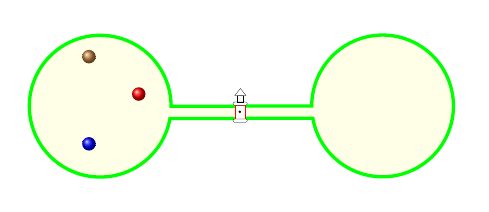
\begin{tikzpicture}[thick,scale=0.9, every node/.style={transform shape}]
\draw [green, very thick,  fill=yellow!10] (0,0) -- ++ (-1,0) arc (0:350:1.0) -- ++ (1,0)   |- cycle ;
\draw [green, very thick,  fill=yellow!10, yshift=.83cm]  (0,-1)-- ++(1,0) arc (190:540:1.0)  -- ++(-1,0)|- cycle ;
\begin{scope}[transform canvas={scale=.1},overlay,shift={(-1,-1.8)}]
\draw [red, fill=white] (0,0) -- ++ (1.5,0)-- ++ (0,1.9)-- ++ (-1.5,0)   |- cycle ;
\draw[rounded corners=5pt, fill=white] (-0.25,1.9) rectangle ++(2,0.5);
\draw[rounded corners=5pt, fill=white] (-0.25,-.5) rectangle ++(2,0.5);
\draw (.7,1) node[circle, draw,fill=black]{};
\draw[xshift=9, yshift=1.4cm]  (0,1) rectangle ++(.8,1);
\draw [black, fill=white,yshift=3.3cm, xshift=-.5] (0,0) -- ++ (.8,1)-- ++ (.8,-1)    |- cycle ;
\shade [ball color=red, shift={(-40em,10em)}] (0:0.5) circle (0.95cm);
\shade [ball color=blue, shift={(-60em,-10em)}] (0:0.5) circle (0.95cm);
\shade [ball color=brown, shift={(-60em,25em)}] (0:0.5) circle (0.95cm);
\end{scope}
\end{tikzpicture}\end{center}
\begin{inparaenum}[(a)]
\item How many arrangements are possible?	%(8)
\item Which is the most likely arrangement?	%spread circles (1,2) or (2,1)
\item Which is the probability of the most likely arrangement?	%(3/8)
\end{inparaenum}
\end{question}
\begin{solution}
\begin{inparaenum}[(a)]
\item  8 
\item  spread circles (1,2) or (2,1)
\item  3/8 
\end{inparaenum}
\hspace{0.1cm}\end{solution}\stepcounter{numA}%%%%%%%%%%%%


\begin{question}[ID=\the\value{numA}]\SetQuestionProperties{section-title=\nameref{sec:units}}
Think about the possible arrangements of four different molecules in a two-bulbed flask:
\begin{center}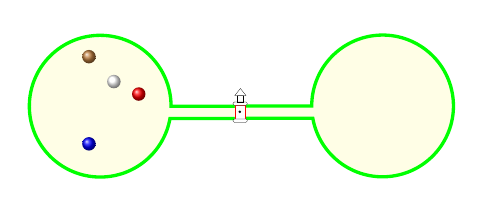
\begin{tikzpicture}[thick,scale=0.9, every node/.style={transform shape}]
\draw [green, very thick,  fill=yellow!10] (0,0) -- ++ (-1,0) arc (0:350:1.0) -- ++ (1,0)   |- cycle ;
\draw [green, very thick,  fill=yellow!10, yshift=.83cm]  (0,-1)-- ++(1,0) arc (190:540:1.0)  -- ++(-1,0)|- cycle ;
\begin{scope}[transform canvas={scale=.1},overlay,shift={(-1,-1.8)}]
\draw [red, fill=white] (0,0) -- ++ (1.5,0)-- ++ (0,1.9)-- ++ (-1.5,0)   |- cycle ;
\draw[rounded corners=5pt, fill=white] (-0.25,1.9) rectangle ++(2,0.5);
\draw[rounded corners=5pt, fill=white] (-0.25,-.5) rectangle ++(2,0.5);
\draw (.7,1) node[circle, draw,fill=black]{};
\draw[xshift=9, yshift=1.4cm]  (0,1) rectangle ++(.8,1);
\draw [black, fill=white,yshift=3.3cm, xshift=-.5] (0,0) -- ++ (.8,1)-- ++ (.8,-1)    |- cycle ;
\shade [ball color=red, shift={(-40em,10em)}] (0:0.5) circle (0.95cm);
\shade [ball color=white, shift={(-50em,15em)}] (0:0.5) circle (0.95cm);
\shade [ball color=blue, shift={(-60em,-10em)}] (0:0.5) circle (0.95cm);
\shade [ball color=brown, shift={(-60em,25em)}] (0:0.5) circle (0.95cm);
\end{scope}
\end{tikzpicture}\end{center}
\begin{inparaenum}[(a)]
\item How many arrangements are possible?	%(16)
\item Which is the most likely arrangement?	%(spread circles)
\item Which is the probability of the most likely arrangement?	%(6/16)
\end{inparaenum}
\end{question}
\begin{solution}
\begin{inparaenum}[(a)]
\item  16 
\item  spread circles (2,2) 
\item  6/16 
\end{inparaenum}
\hspace{0.1cm}\end{solution}\stepcounter{numA}%%%%%%%%%%%%






\end{multicols*}

\newpage
\begin{answersenvironment}
\begin{minipage}[c]{1\textwidth}
\begin{localsize}{10}
{\Large \bf Answers}
\SetupExSheets{
  headings = inline-nr , % numbered and inline
  counter-format = qu) , % numbers 1) 2) ... 
}
%\printsolutions 
 % \printsolutions[byID={1,3,5,7,9,11,13,15,17,19,21,23,25,27,29,31,33,35,37}]
\end{localsize}
\end{minipage}\end{answersenvironment}
\end{document}

